% \VignetteIndexEntry{mAPKL Tutorial}
% \VignetteKeywords{Microarray feature selection}
% \VignettePackage{mAPKL}
% \VignetteEngine{knitr::knitr}

\documentclass[12pt]{article}\usepackage[]{graphicx}\usepackage[usenames,dvipsnames]{color}
%% maxwidth is the original width if it is less than linewidth
%% otherwise use linewidth (to make sure the graphics do not exceed the margin)
\makeatletter
\def\maxwidth{ %
  \ifdim\Gin@nat@width>\linewidth
    \linewidth
  \else
    \Gin@nat@width
  \fi
}
\makeatother

\definecolor{fgcolor}{rgb}{0.345, 0.345, 0.345}
\newcommand{\hlnum}[1]{\textcolor[rgb]{0.686,0.059,0.569}{#1}}%
\newcommand{\hlstr}[1]{\textcolor[rgb]{0.192,0.494,0.8}{#1}}%
\newcommand{\hlcom}[1]{\textcolor[rgb]{0.678,0.584,0.686}{\textit{#1}}}%
\newcommand{\hlopt}[1]{\textcolor[rgb]{0,0,0}{#1}}%
\newcommand{\hlstd}[1]{\textcolor[rgb]{0.345,0.345,0.345}{#1}}%
\newcommand{\hlkwa}[1]{\textcolor[rgb]{0.161,0.373,0.58}{\textbf{#1}}}%
\newcommand{\hlkwb}[1]{\textcolor[rgb]{0.69,0.353,0.396}{#1}}%
\newcommand{\hlkwc}[1]{\textcolor[rgb]{0.333,0.667,0.333}{#1}}%
\newcommand{\hlkwd}[1]{\textcolor[rgb]{0.737,0.353,0.396}{\textbf{#1}}}%
\let\hlipl\hlkwb

\usepackage{framed}
\makeatletter
\newenvironment{kframe}{%
 \def\at@end@of@kframe{}%
 \ifinner\ifhmode%
  \def\at@end@of@kframe{\end{minipage}}%
  \begin{minipage}{\columnwidth}%
 \fi\fi%
 \def\FrameCommand##1{\hskip\@totalleftmargin \hskip-\fboxsep
 \colorbox{shadecolor}{##1}\hskip-\fboxsep
     % There is no \\@totalrightmargin, so:
     \hskip-\linewidth \hskip-\@totalleftmargin \hskip\columnwidth}%
 \MakeFramed {\advance\hsize-\width
   \@totalleftmargin\z@ \linewidth\hsize
   \@setminipage}}%
 {\par\unskip\endMakeFramed%
 \at@end@of@kframe}
\makeatother

\definecolor{shadecolor}{rgb}{.97, .97, .97}
\definecolor{messagecolor}{rgb}{0, 0, 0}
\definecolor{warningcolor}{rgb}{1, 0, 1}
\definecolor{errorcolor}{rgb}{1, 0, 0}
\newenvironment{knitrout}{}{} % an empty environment to be redefined in TeX

\usepackage{alltt}

\RequirePackage{C:/Users/argi/Documents/R/win-library/3.3/BiocStyle/resources/tex/Bioconductor}

\AtBeginDocument{\bibliographystyle{C:/Users/argi/Documents/R/win-library/3.3/BiocStyle/resources/tex/unsrturl}}


\usepackage{microtype}
\usepackage{amsmath}
\usepackage{amssymb}
\usepackage{graphicx}

\newcommand*\rfrac[2]{{}^{#1}\!/_{#2}}
\IfFileExists{upquote.sty}{\usepackage{upquote}}{}
\begin{document}



\title{Bioconductor mAPKL Package}
\author{Argiris Sakellariou$^{1,2}$\\[1cm]
\small{$^1$ Biomedical Informatics Unit, Biomedical Research Foundation of the 
Academy of Athens, Athens, Greece}\\[0cm]
\small{$^2$ Department of Informatics and Telecommunications, National and 
Kapodistrian Univ. of Athens, Athens, Greece}\\[0cm]
\texttt{\small{argisake@gmail.com}}
}

\maketitle
\pagenumbering{roman}

\renewcommand{\baselinestretch}{1.2}
\tableofcontents

\pagenumbering{arabic}
\setcounter{page}{1}

\section{Introduction}
\noindent The mAPKL bioconductor R package implements a hybrid gene selection 
method, which is based on the hypothesis that among the statistically 
significant genes in a ranked list, there should be clusters of genes that share
similar biological functions related to the investigated disease.Thus, instead 
of keeping a number of $N$ top ranked genes, it would be more appropriate to 
define and keep a number of gene cluster exemplars. 

\noindent The proposed methodology combines filtering and cluster analysis to 
select a small  yet highly discriminatory set of non-redundant genes. Regarding 
the filtering step, a multiple hypothesis testing approach from \emph{multtest} 
r-package (maxT) is employed to rank the genes of the training set according to 
their differential expression.Then the top N genes (e.g. N = 200) are reserved 
for cluster analysis. First the index of Krzanowski and Lai as included in the 
\emph{ClusterSim} r-package is applied on the disease samples of the training 
set to determine the number of clusters. The Krzanowski and Lai index is defined 
by $DIFF(k)=(k-1)^\frac{2}{p}W_{k-1}-k^\frac{2}{p}W_{k}$ when choosing the 
number of clusters $(k)$ to maximize the 
quantity $KL(k)=\Big|\frac{DIFF(k)}{DIFF_(k+1)}\Big|$.
The $W_k$ denotes the within-cluster sum of squared errors. 

\noindent Finally, cluster analysis is performed with the aid of Affinity 
Propagation (AP) clustering algorithm, which detects $n (n=k$ the Krzanowski 
and Lai index) clusters among the top $N$ genes, the so called exemplars.Those 
$n$ exemplars are expected to form a classifier that shall discriminate between 
normal and disease samples (Sakellariou et al. 2012, \emph{BMC Bioinformatics} 
\textbf{13}:270).
\noindent This package implements the pre-mentioned methodology through a core 
function, the \emph{mAPKL}. In the upcoming sections follows a guidance of the 
included functions and its functionality through differential expression 
analysis scenarios on a breast cancer dataset (GSE5764) which is part of the 
\emph{mAPKLData} package.

\section{Identification of deferentially expressed genes}
\subsection{Breast cancer data}
\noindent Throught this tutorial we utilized a publicly available breast cancer 
dataset comprised of 30 samples, where 20 of them represent normal cases and the 
remaining 10 samples  stand for tumor cases. We first load the package and then 
the breast cancer data. Then with the aid of the \emph{sampling} function we  
create a separate training and validation sets where 60\% of the samples will 
be used for training and the rest 40\% of the samples will 
be used for evaluation purposes.

\begin{knitrout}
\definecolor{shadecolor}{rgb}{0.969, 0.969, 0.969}\color{fgcolor}\begin{kframe}
\begin{alltt}
\hlkwd{library}\hlstd{(mAPKL)}
\hlkwd{library}\hlstd{(mAPKLData)}
\hlkwd{data}\hlstd{(mAPKLData)}
\hlkwd{varLabels}\hlstd{(mAPKLData)}
\hlstd{breast} \hlkwb{<-} \hlkwd{sampling}\hlstd{(}\hlkwc{Data}\hlstd{=mAPKLData,} \hlkwc{valPercent}\hlstd{=}\hlnum{40}\hlstd{,} \hlkwc{classLabels}\hlstd{=}\hlstr{"type"}\hlstd{,} \hlkwc{seed}\hlstd{=}\hlnum{135}\hlstd{)}
\end{alltt}
\end{kframe}
\end{knitrout}

\noindent The \emph{sampling} function returns an S3 class (breast) with two 
eSet class objects that nest the relevant training and validation sampes. Those 
two objects are used throughout the rest of the analysis.

\begin{knitrout}
\definecolor{shadecolor}{rgb}{0.969, 0.969, 0.969}\color{fgcolor}\begin{kframe}
\begin{alltt}
\hlstd{breast}
\end{alltt}
\begin{verbatim}
## $trainData
## ExpressionSet (storageMode: lockedEnvironment)
## assayData: 54675 features, 18 samples 
##   element names: exprs 
## protocolData: none
## phenoData
##   sampleNames: GSM134584 GSM134690 ... GSM134695 (18 total)
##   varLabels: title type
##   varMetadata: labelDescription
## featureData: none
## experimentData: use 'experimentData(object)'
##   pubMedIds: 17389037 
## Annotation: hgu133plus2 
## 
## $testData
## ExpressionSet (storageMode: lockedEnvironment)
## assayData: 54675 features, 12 samples 
##   element names: exprs 
## protocolData: none
## phenoData
##   sampleNames: GSM134691 GSM134588 ... GSM134692 (12 total)
##   varLabels: title type
##   varMetadata: labelDescription
## featureData: none
## experimentData: use 'experimentData(object)'
##   pubMedIds: 17389037 
## Annotation: hgu133plus2
\end{verbatim}
\end{kframe}
\end{knitrout}

\subsection{Data normalization and transformation}
\noindent We perform normalization to the expression values through the 
\emph{preprocess} function.

\begin{knitrout}
\definecolor{shadecolor}{rgb}{0.969, 0.969, 0.969}\color{fgcolor}\begin{kframe}
\begin{alltt}
\hlstd{normTrainData} \hlkwb{<-} \hlkwd{preprocess}\hlstd{(breast}\hlopt{$}\hlstd{trainData)}
\hlstd{normTestData} \hlkwb{<-} \hlkwd{preprocess}\hlstd{(breast}\hlopt{$}\hlstd{testData)}
\end{alltt}
\end{kframe}
\end{knitrout}

\noindent The \emph{preprocess} function produces a list of several available 
normalization and transformation options. Besides density plots per method are 
produced and saved to current working directory to assist the user to decide 
upon which method to select before proceeding to mAPKL analysis.

\begin{knitrout}
\definecolor{shadecolor}{rgb}{0.969, 0.969, 0.969}\color{fgcolor}\begin{kframe}
\begin{alltt}
\hlkwd{attributes}\hlstd{(normTrainData)}
\end{alltt}
\begin{verbatim}
## $names
## [1] "rawdata"       "mc.normdata"   "z.normdata"    "q.normdata"    "cl.normdata"  
## [6] "mcL2.normdata" "zL2.normdata"  "qL2.normdata"  "clL2.normdata"
\end{verbatim}
\end{kframe}
\end{knitrout}

\noindent The following graph presents the density plots of 8 possible 
normalization process with or without log2 transformation. The \emph{preprocess} 
function applies all of them and it is up to the user, which one will engage for 
the rest of the analysis. In brief, the available approaches are mean-centering, 
z-score, quantile, and cyclic loess. 
During this case study we will proceed with the expression values folowing log2 
transformation and cyclic loess normalization.

\begin{figure}[]
\centering
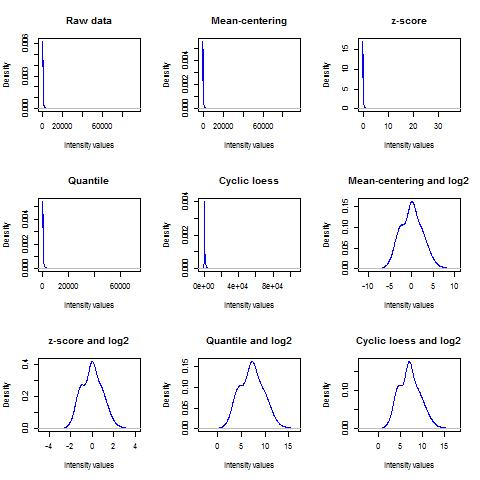
\includegraphics[width=15cm,height=15cm,keepaspectratio]{../man/figures/density_train}
\caption{Density plots of normalized intensity values}
\end{figure}

\subsection{mAPKL gene selection}
\noindent In this example we employ the expresion values of log2 transformation 
and cyclic loess normalization to proceed with the \emph{mAPKL} analysis.

\begin{knitrout}
\definecolor{shadecolor}{rgb}{0.969, 0.969, 0.969}\color{fgcolor}\begin{kframe}
\begin{alltt}
\hlkwd{exprs}\hlstd{(breast}\hlopt{$}\hlstd{trainData)} \hlkwb{<-} \hlstd{normTrainData}\hlopt{$}\hlstd{clL2.normdata}
\hlkwd{exprs}\hlstd{(breast}\hlopt{$}\hlstd{testData)} \hlkwb{<-} \hlstd{normTestData}\hlopt{$}\hlstd{clL2.normdata}
\hlstd{out.clL2} \hlkwb{<-} \hlkwd{mAPKL}\hlstd{(}\hlkwc{trObj} \hlstd{= breast}\hlopt{$}\hlstd{trainData,} \hlkwc{classLabels} \hlstd{=} \hlstr{"type"}\hlstd{,}
    \hlkwc{valObj} \hlstd{= breast}\hlopt{$}\hlstd{testData,} \hlkwc{dataType} \hlstd{=} \hlnum{7}\hlstd{)}
\end{alltt}
\begin{verbatim}
## b=10	b=20	b=30	b=40	b=50	b=60	b=70	b=80	b=90	b=100	
## b=110	b=120	b=130	b=140	b=150	b=160	b=170	b=180	b=190	b=200	
## b=210	b=220	b=230	b=240	b=250	b=260	b=270	b=280	b=290	b=300	
## b=310	b=320	b=330	b=340	b=350	b=360	b=370	b=380	b=390	b=400	
## b=410	b=420	b=430	b=440	b=450	b=460	b=470	b=480	b=490	b=500	
## b=510	b=520	b=530	b=540	b=550	b=560	b=570	b=580	b=590	b=600	
## b=610	b=620	b=630	b=640	b=650	b=660	b=670	b=680	b=690	b=700	
## b=710	b=720	b=730	b=740	b=750	b=760	b=770	b=780	b=790	b=800	
## b=810	b=820	b=830	b=840	b=850	b=860	b=870	b=880	b=890	b=900	
## b=910	b=920	b=930	b=940	b=950	b=960	b=970	b=980	b=990	b=1000	
\end{verbatim}


{\ttfamily\noindent\itshape\color{messagecolor}{\#\# Please wait! The (KL) cluster indexing may take several minutes...}}

{\ttfamily\noindent\itshape\color{messagecolor}{\#\# Asking for 15 number of clusters}}

{\ttfamily\noindent\itshape\color{messagecolor}{\#\# fc according to limma}}\end{kframe}
\end{knitrout}

\subsection{Building and evaluating classification models}
\noindent  After having get the exemplars from \emph{mAPKL} analysis we build an 
SVM classifier to test their discriminatory performance. Regarding the SVM 
setup, we utilize a linear kernel for which the cost attribute is infered by the 
tune.svm function. however, the user may freely use another kernel and a 
different Cross Validation approach than 5-folds.

\begin{knitrout}
\definecolor{shadecolor}{rgb}{0.969, 0.969, 0.969}\color{fgcolor}\begin{kframe}
\begin{alltt}
\hlstd{clasPred} \hlkwb{<-} \hlkwd{classification}\hlstd{(out.clL2}\hlopt{@}\hlkwc{exemplTrain}\hlstd{,} \hlstr{"type"}\hlstd{, out.clL2}\hlopt{@}\hlkwc{exemplTest}\hlstd{)}
\end{alltt}


{\ttfamily\noindent\itshape\color{messagecolor}{\#\# The training set has 12 Negative and 6 Positive samples. Using k-fold=5 C-V}}

{\ttfamily\noindent\itshape\color{messagecolor}{\#\# \#\#\#\#\#\#\#\#\#\#\#\# THE BEST PARAMETERS TUNING STAGE \#\#\#\#\#\#\#\#\#\#\#\#\#\#\#\#\#\#}}

{\ttfamily\noindent\itshape\color{messagecolor}{\#\# \#\#\#\#\#\#\#\#\#\#\#\#\# THE TRAINING STAGE \#\#\#\#\#\#\#\#\#\#\#\#\#\#\#\#\#\#\#\#\#\#\#\#}}\begin{verbatim}
## 
## Call:
## svm.default(x = train.mtx, y = lbls, scale = FALSE, type = "C-classification", 
##     kernel = "linear", gamma = best_gamma, cost = best_cost, cross = k_fold)
## 
## 
## Parameters:
##    SVM-Type:  C-classification 
##  SVM-Kernel:  linear 
##        cost:  2 
##       gamma:  0.125 
## 
## Number of Support Vectors:  5
\end{verbatim}


{\ttfamily\noindent\itshape\color{messagecolor}{\#\# \#\#\#\#\#\#\#\#\#\#\#\#\# THE PREDICTION STAGE \#\#\#\#\#\#\#\#\#\#\#\#\#\#\#\#\#\#\#\#\#\#}}\begin{verbatim}
##           Test Labels Prediction Labels
## GSM134691           0                 0
## GSM134588           0                 0
## GSM134688           0                 0
## GSM134694           0                 1
## GSM134697           0                 0
## GSM134700           0                 0
## GSM134687           0                 0
## GSM134709           0                 0
## GSM134710           1                 1
## GSM134698           1                 1
## GSM134689           1                 1
## GSM134692           1                 1
\end{verbatim}


{\ttfamily\noindent\itshape\color{messagecolor}{\#\# Negative samples: 8}}

{\ttfamily\noindent\itshape\color{messagecolor}{\#\# Positive samples: 4}}

{\ttfamily\noindent\itshape\color{messagecolor}{\#\# TN=7}}

{\ttfamily\noindent\itshape\color{messagecolor}{\#\# FP=1}}

{\ttfamily\noindent\itshape\color{messagecolor}{\#\# TP=4}}

{\ttfamily\noindent\itshape\color{messagecolor}{\#\# FN=0}}

{\ttfamily\noindent\itshape\color{messagecolor}{\#\# AUC=0.94}}

{\ttfamily\noindent\itshape\color{messagecolor}{\#\# Accuracy=92.00}}

{\ttfamily\noindent\itshape\color{messagecolor}{\#\# MCC=0.84}}

{\ttfamily\noindent\itshape\color{messagecolor}{\#\# Specificity=0.88}}

{\ttfamily\noindent\itshape\color{messagecolor}{\#\# Sensitivity=1.00}}\end{kframe}
\end{knitrout}

\noindent  The output of the \emph{classification} inform us about the SVM set 
up, the number of Support Vectors and finally show the the predicted labels 
along with the initial. In this example there is a validation set different from 
the training set and therefore we may use the respective labels to obtain the 
performance characteristcs. The relevant function \emph{metrics} called inside 
the \emph{classification} function, calculates five key meassures: the Area 
Under the ROC curve AUC, the classification accuracy, the Matthews correlation 
coefficient MCC classification meassure, the degree of true negative's 
identification Specificity, and finally the degree of true positive's 
identification Sensitivity.

\section{Advanced usage of the package}
\subsection{Annotation analysis}
\noindent  For each contemporary chip technology, there is a relevant annotation 
file, in which the the user may drag several \emph{genome oriented} information. 
Regarding the breast cancer microarray data, the gene expression values were 
stored on Affumetrix gene chips. Using the \emph{annotate} function, the user 
may obtain several info related to probe id, gene symbol, Entrez id, ensembl id, 
and chromosomal location.

\begin{knitrout}
\definecolor{shadecolor}{rgb}{0.969, 0.969, 0.969}\color{fgcolor}\begin{kframe}
\begin{alltt}
\hlstd{gene.info} \hlkwb{<-} \hlkwd{annotate}\hlstd{(out.clL2}\hlopt{@}\hlkwc{exemplars}\hlstd{,} \hlstr{"hgu133plus2.db"}\hlstd{)}
\hlstd{gene.info}\hlopt{@}\hlkwc{results}
\end{alltt}
\begin{verbatim}
##         PROBEID       SYMBOL  ENTREZID         ENSEMBL      MAP
## 1   215717_s_at         FBN2      2201 ENSG00000138829   5q23.3
## 2    1561358_at        TXLNA    200081 ENSG00000084652   1p35.1
## 3   222752_s_at      TMEM206     55248 ENSG00000065600   1q32.3
## 4     233922_at         <NA>      <NA>            <NA>     <NA>
## 5   218871_x_at   CSGALNACT2     55454 ENSG00000169826 10q11.21
## 6    33323_r_at          SFN      2810 ENSG00000175793  1p36.11
## 7     244311_at         <NA>      <NA>            <NA>     <NA>
## 8     220932_at         <NA>      <NA>            <NA>     <NA>
## 9     205508_at        SCN1B      6324 ENSG00000105711  19q13.1
## 10    209596_at        MXRA5     25878 ENSG00000101825  Xp22.33
## 11    215180_at         <NA>      <NA>            <NA>     <NA>
## 12 1560638_a_at LOC105375839 105375839            <NA>     <NA>
## 13  201852_x_at       COL3A1      1281 ENSG00000168542     2q31
## 14    229947_at         PI15     51050 ENSG00000137558  8q21.11
## 15  221731_x_at         VCAN      1462 ENSG00000038427   5q14.3
\end{verbatim}
\end{kframe}
\end{knitrout}

\noindent  We may exploit the output of the \emph{annotate} function to extent 
our analysis. For instance, we may perform \emph{pathway analysis} on the 
exemplars. For this purpose we will utilize the \emph{probes2pathways} function that utilizes the \emph{reactome.db} package.This function employs the probe ids to identify the relevant pathways.

\begin{knitrout}
\definecolor{shadecolor}{rgb}{0.969, 0.969, 0.969}\color{fgcolor}\begin{kframe}
\begin{alltt}
\hlkwd{probes2pathways}\hlstd{(gene.info)}
\end{alltt}
\begin{verbatim}
##                                                 14742281 
##  "Homo sapiens: Degradation of the extracellular matrix" 
##                                                 14742282 
##  "Homo sapiens: Degradation of the extracellular matrix" 
##                                                 15669481 
##                  "Homo sapiens: Elastic fibre formation" 
##                                                 15669482 
##                  "Homo sapiens: Elastic fibre formation" 
##                                                 14742441 
##        "Homo sapiens: Extracellular matrix organization" 
##                                                 14742442 
##        "Homo sapiens: Extracellular matrix organization" 
##                                                 21293791 
## "Homo sapiens: Molecules associated with elastic fibres" 
##                                                 21293792 
## "Homo sapiens: Molecules associated with elastic fibres" 
##                                                 14742281 
##  "Homo sapiens: Degradation of the extracellular matrix" 
##                                                 14742282 
##  "Homo sapiens: Degradation of the extracellular matrix" 
##                                                 15669481 
##                  "Homo sapiens: Elastic fibre formation" 
##                                                 15669482 
##                  "Homo sapiens: Elastic fibre formation" 
##                                                 14742441 
##        "Homo sapiens: Extracellular matrix organization" 
##                                                 14742442 
##        "Homo sapiens: Extracellular matrix organization" 
##                                                 21293791 
## "Homo sapiens: Molecules associated with elastic fibres" 
##                                                 21293792 
## "Homo sapiens: Molecules associated with elastic fibres"
\end{verbatim}
\end{kframe}
\end{knitrout}

\subsection{Network characteristics}
\noindent  Regarding the network charcteristics, we compute through the 
\emph{netwAttr} function three different types of centralities 
(degree, closeness, betweenness) and a meassure for clustering coefficient 
called transitivity. The degree centrality of a node refer to the number of 
connections or edges of that node to other nodes.The closeness centrality 
describes the reciprocal accumulated shortest length distance from a node to all 
other connected nodes.The betweeness centrality depicts the number of times a 
node intervenes along the shortest path of two other nodes. Transitivity 
meassures the degree of nodes to create clusters within a network.For all four 
network meassures we provide both global and local values. Furthermore, we 
compose an edge list (Node1-Node2-weight) based on the \emph{N} top ranked genes.
\noindent  We may exploit that meassures to depict the exemplars' network 
characteristics
\begin{knitrout}
\definecolor{shadecolor}{rgb}{0.969, 0.969, 0.969}\color{fgcolor}\begin{kframe}
\begin{alltt}
\hlstd{net.attr} \hlkwb{<-} \hlkwd{netwAttr}\hlstd{(out.clL2)}
\hlstd{wDegreeL} \hlkwb{<-} \hlstd{net.attr}\hlopt{@}\hlkwc{degree}\hlopt{$}\hlstd{WdegreeL[out.clL2}\hlopt{@}\hlkwc{exemplars}\hlstd{]}
\hlstd{wClosenessL} \hlkwb{<-} \hlstd{net.attr}\hlopt{@}\hlkwc{closeness}\hlopt{$}\hlstd{WclosenessL[out.clL2}\hlopt{@}\hlkwc{exemplars}\hlstd{]}
\hlstd{wBetweenessL} \hlkwb{<-} \hlstd{net.attr}\hlopt{@}\hlkwc{betweenness}\hlopt{$}\hlstd{WbetweennessL[out.clL2}\hlopt{@}\hlkwc{exemplars}\hlstd{]}
\hlstd{wTransitivityL} \hlkwb{<-} \hlstd{net.attr}\hlopt{@}\hlkwc{transitivity}\hlopt{$}\hlstd{WtransitivityL[out.clL2}\hlopt{@}\hlkwc{exemplars}\hlstd{]}
\end{alltt}
\end{kframe}
\end{knitrout}
\begin{knitrout}
\definecolor{shadecolor}{rgb}{0.969, 0.969, 0.969}\color{fgcolor}\begin{kframe}
\begin{alltt}
\hlstd{Global.val} \hlkwb{<-} \hlkwd{c}\hlstd{(net.attr}\hlopt{@}\hlkwc{degree}\hlopt{$}\hlstd{WdegreeG, net.attr}\hlopt{@}\hlkwc{closeness}\hlopt{$}\hlstd{WclosenessG,}
    \hlstd{net.attr}\hlopt{@}\hlkwc{betweenness}\hlopt{$}\hlstd{WbetweennessG, net.attr}\hlopt{@}\hlkwc{transitivity}\hlopt{$}\hlstd{WtransitivityG)}
\end{alltt}
\end{kframe}
\end{knitrout}
\begin{knitrout}
\definecolor{shadecolor}{rgb}{0.969, 0.969, 0.969}\color{fgcolor}\begin{kframe}
\begin{alltt}
\hlstd{Global.val} \hlkwb{<-} \hlkwd{round}\hlstd{(Global.val,} \hlnum{2}\hlstd{)}
\hlstd{exempl.netattr} \hlkwb{<-} \hlkwd{rbind}\hlstd{(wDegreeL, wClosenessL, wBetweenessL, wTransitivityL)}
\end{alltt}
\end{kframe}
\end{knitrout}
\begin{knitrout}
\definecolor{shadecolor}{rgb}{0.969, 0.969, 0.969}\color{fgcolor}\begin{kframe}
\begin{alltt}
\hlstd{netAttr} \hlkwb{<-} \hlkwd{cbind}\hlstd{(Global.val, exempl.netattr)}
\hlstd{netAttr} \hlkwb{<-} \hlkwd{t}\hlstd{(netAttr)}
\hlstd{netAttr}
\end{alltt}
\begin{verbatim}
##              wDegreeL wClosenessL wBetweenessL wTransitivityL
## Global.val     330.18        0.93       741.81           0.57
## 215717_s_at    308.35        1.25       886.00           0.14
## 1561358_at     346.92        1.34      1141.00           0.14
## 222752_s_at    327.89        0.65         0.00           0.14
## 233922_at      317.58        0.79         2.00           0.15
## 218871_x_at    293.73        0.53       768.00           0.14
## 33323_r_at     338.19        0.27         0.00           0.13
## 244311_at      294.80        0.63         0.00           0.15
## 220932_at      359.10        0.66         0.00           0.14
## 205508_at      309.07        0.89         4.00           0.14
## 209596_at      345.13        1.34       278.00           0.14
## 215180_at      333.37        1.37      1440.00           0.14
## 1560638_a_at   368.23        1.38      4615.00           0.14
## 201852_x_at    353.34        0.93        24.67           0.15
## 229947_at      317.11        1.19       496.00           0.15
## 221731_x_at    331.01        0.61        14.00           0.15
\end{verbatim}
\end{kframe}
\end{knitrout}

\noindent and identify potential hubs.The calculations of this example are based on the "clr" network reconstruction method. However, there are for the time being two more options, including the "aracne.a" and "aracne.m".
\begin{knitrout}
\definecolor{shadecolor}{rgb}{0.969, 0.969, 0.969}\color{fgcolor}\begin{kframe}
\begin{alltt}
\hlcom{# For local degree > global + standard deviation}
\hlstd{sdev} \hlkwb{<-} \hlkwd{sd}\hlstd{(net.attr}\hlopt{@}\hlkwc{degree}\hlopt{$}\hlstd{WdegreeL)}
\hlstd{msd} \hlkwb{<-} \hlstd{net.attr}\hlopt{@}\hlkwc{degree}\hlopt{$}\hlstd{WdegreeG} \hlopt{+} \hlstd{sdev}
\hlstd{hubs} \hlkwb{<-} \hlstd{wDegreeL[}\hlkwd{which}\hlstd{(wDegreeL} \hlopt{>} \hlstd{msd)]}
\hlstd{hubs}
\end{alltt}
\begin{verbatim}
##    220932_at 1560638_a_at 
##       359.10       368.23
\end{verbatim}
\end{kframe}
\end{knitrout}

\noindent Finally, we may plot the network for those nodes that their local 
weighted degree is greater than Global weithed degree plus 2 times the standard 
deviation. We set  this rule for both significance and illustartion purposes 
(that edge list has dimension 604 x 3).
\vfill
\begin{figure}[]
\centering
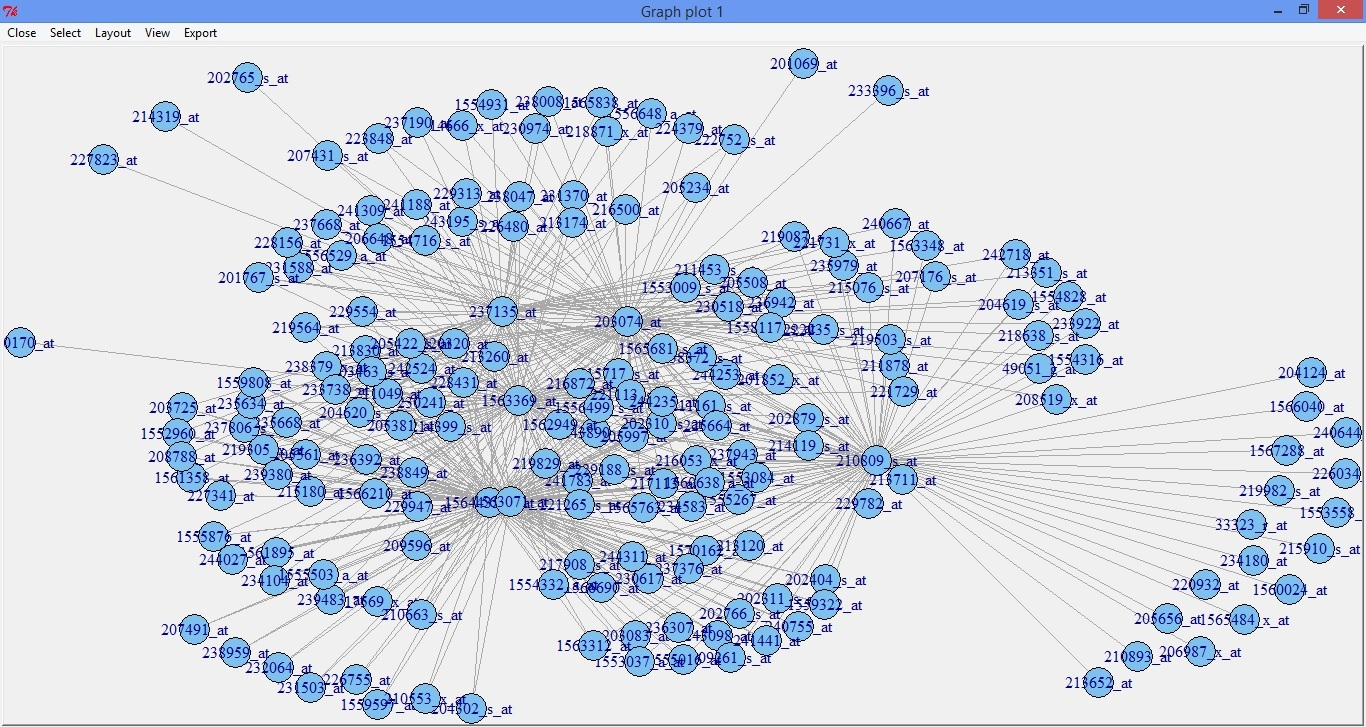
\includegraphics[width=15cm,height=15cm,keepaspectratio]{../man/figures/network}
\caption{Degree centrality network}
\end{figure}

\begin{knitrout}
\definecolor{shadecolor}{rgb}{0.969, 0.969, 0.969}\color{fgcolor}\begin{kframe}
\begin{alltt}
\hlstd{sdev} \hlkwb{<-} \hlkwd{sd}\hlstd{(net.attr}\hlopt{@}\hlkwc{degree}\hlopt{$}\hlstd{WdegreeL)}
\hlstd{ms2d} \hlkwb{<-} \hlstd{net.attr}\hlopt{@}\hlkwc{degree}\hlopt{$}\hlstd{WdegreeG} \hlopt{+} \hlnum{2} \hlopt{*} \hlstd{sdev}
\hlstd{net} \hlkwb{<-} \hlstd{net.attr}\hlopt{@}\hlkwc{degree}\hlopt{$}\hlstd{WdegreeL[}\hlkwd{which}\hlstd{(net.attr}\hlopt{@}\hlkwc{degree}\hlopt{$}\hlstd{WdegreeL} \hlopt{>}
    \hlstd{ms2d)]}
\hlstd{idx} \hlkwb{<-} \hlkwd{which}\hlstd{(net.attr}\hlopt{@}\hlkwc{edgelist}\hlstd{[,} \hlnum{1}\hlstd{]} \hlopt \hlkwd{names}\hlstd{(net))}
\hlstd{new.edgeList} \hlkwb{<-} \hlstd{net.attr}\hlopt{@}\hlkwc{edgelist}\hlstd{[idx, ]}
\hlkwd{dim}\hlstd{(new.edgeList)}
\end{alltt}
\begin{verbatim}
## [1] 604   3
\end{verbatim}
\begin{alltt}
\hlkwd{require}\hlstd{(igraph)}
\hlstd{g} \hlkwb{=} \hlkwd{graph.data.frame}\hlstd{(new.edgeList,} \hlkwc{directed} \hlstd{=} \hlnum{FALSE}\hlstd{)}
\hlcom{# tkplot(g,layout=layout.fruchterman.reingold)}
\end{alltt}
\end{kframe}
\end{knitrout}
\vfill
\section{Reporting}
\noindent The overall analysis is summarized in an \textbf{html} report produced 
by the \emph{report} function. It covers the dataset repsresentation depicting 
the samples' names and their respective class labels, the exemplars section 
where statistical results and network characteristcs are included. The 
classification performance section illustrates the performance metrics achieved 
in either cross-validation or hold-out validation.Finally, several annotation 
info are presented if an annotation analysis has occured.

\section{Session info}
\begin{knitrout}
\definecolor{shadecolor}{rgb}{0.969, 0.969, 0.969}\color{fgcolor}\begin{kframe}
\begin{alltt}
\hlkwd{sessionInfo}\hlstd{()}
\end{alltt}
\begin{verbatim}
## R version 3.3.1 (2016-06-21)
## Platform: x86_64-w64-mingw32/x64 (64-bit)
## Running under: Windows 10 x64 (build 14393)
## 
## locale:
## [1] LC_COLLATE=English_United States.1252  LC_CTYPE=English_United States.1252   
## [3] LC_MONETARY=English_United States.1252 LC_NUMERIC=C                          
## [5] LC_TIME=English_United States.1252    
## 
## attached base packages:
## [1] stats4    parallel  stats     graphics  grDevices utils     datasets  methods  
## [9] base     
## 
## other attached packages:
##  [1] igraph_1.0.1         hgu133plus2.db_3.2.3 org.Hs.eg.db_3.4.0   AnnotationDbi_1.35.5
##  [5] IRanges_2.7.17       S4Vectors_0.11.19    mAPKLData_1.5.2      mAPKL_1.5.2         
##  [9] Biobase_2.33.4       BiocGenerics_0.19.2  knitr_1.14          
## 
## loaded via a namespace (and not attached):
##  [1] Rcpp_0.12.7        formatR_1.4        highr_0.6          class_7.3-14      
##  [5] tools_3.3.1        digest_0.6.10      parmigene_1.0.2    jsonlite_1.1      
##  [9] evaluate_0.10      RSQLite_1.0.0      lattice_0.20-34    Matrix_1.2-7.1    
## [13] shiny_0.14.1       DBI_0.5-1          R2HTML_2.3.2       e1071_1.6-7       
## [17] apcluster_1.4.3    stringr_1.1.0      cluster_2.0.5      htmlwidgets_0.7   
## [21] ade4_1.7-4         multtest_2.29.0    grid_3.3.1         modeest_2.1       
## [25] R6_2.2.0           rgl_0.96.0         survival_2.39-5    limma_3.29.22     
## [29] reactome.db_1.55.0 magrittr_1.5       htmltools_0.3.5    MASS_7.3-45       
## [33] splines_3.3.1      BiocStyle_2.1.34   mime_0.5           xtable_1.8-2      
## [37] httpuv_1.3.3       stringi_1.1.2      clusterSim_0.44-5
\end{verbatim}
\end{kframe}
\end{knitrout}

\section{Reference}
\begin{list}{}{\itemindent=-1.0cm}

\item Sakellariou, A., D. Sanoudou, and G. Spyrou. "Combining Multiple 
Hypothesis Testing and Affinity Propagation Clustering Leads to Accurate, 
Robust and Sample Size Independent Classification on Gene Expression Data.
" BMC Bioinformatics 13 (2012): 270.
\item http://www.ncbi.nlm.nih.gov/geo/query/acc.cgi?acc=GSE5764

\end{list}

\begin{figure}
\centering
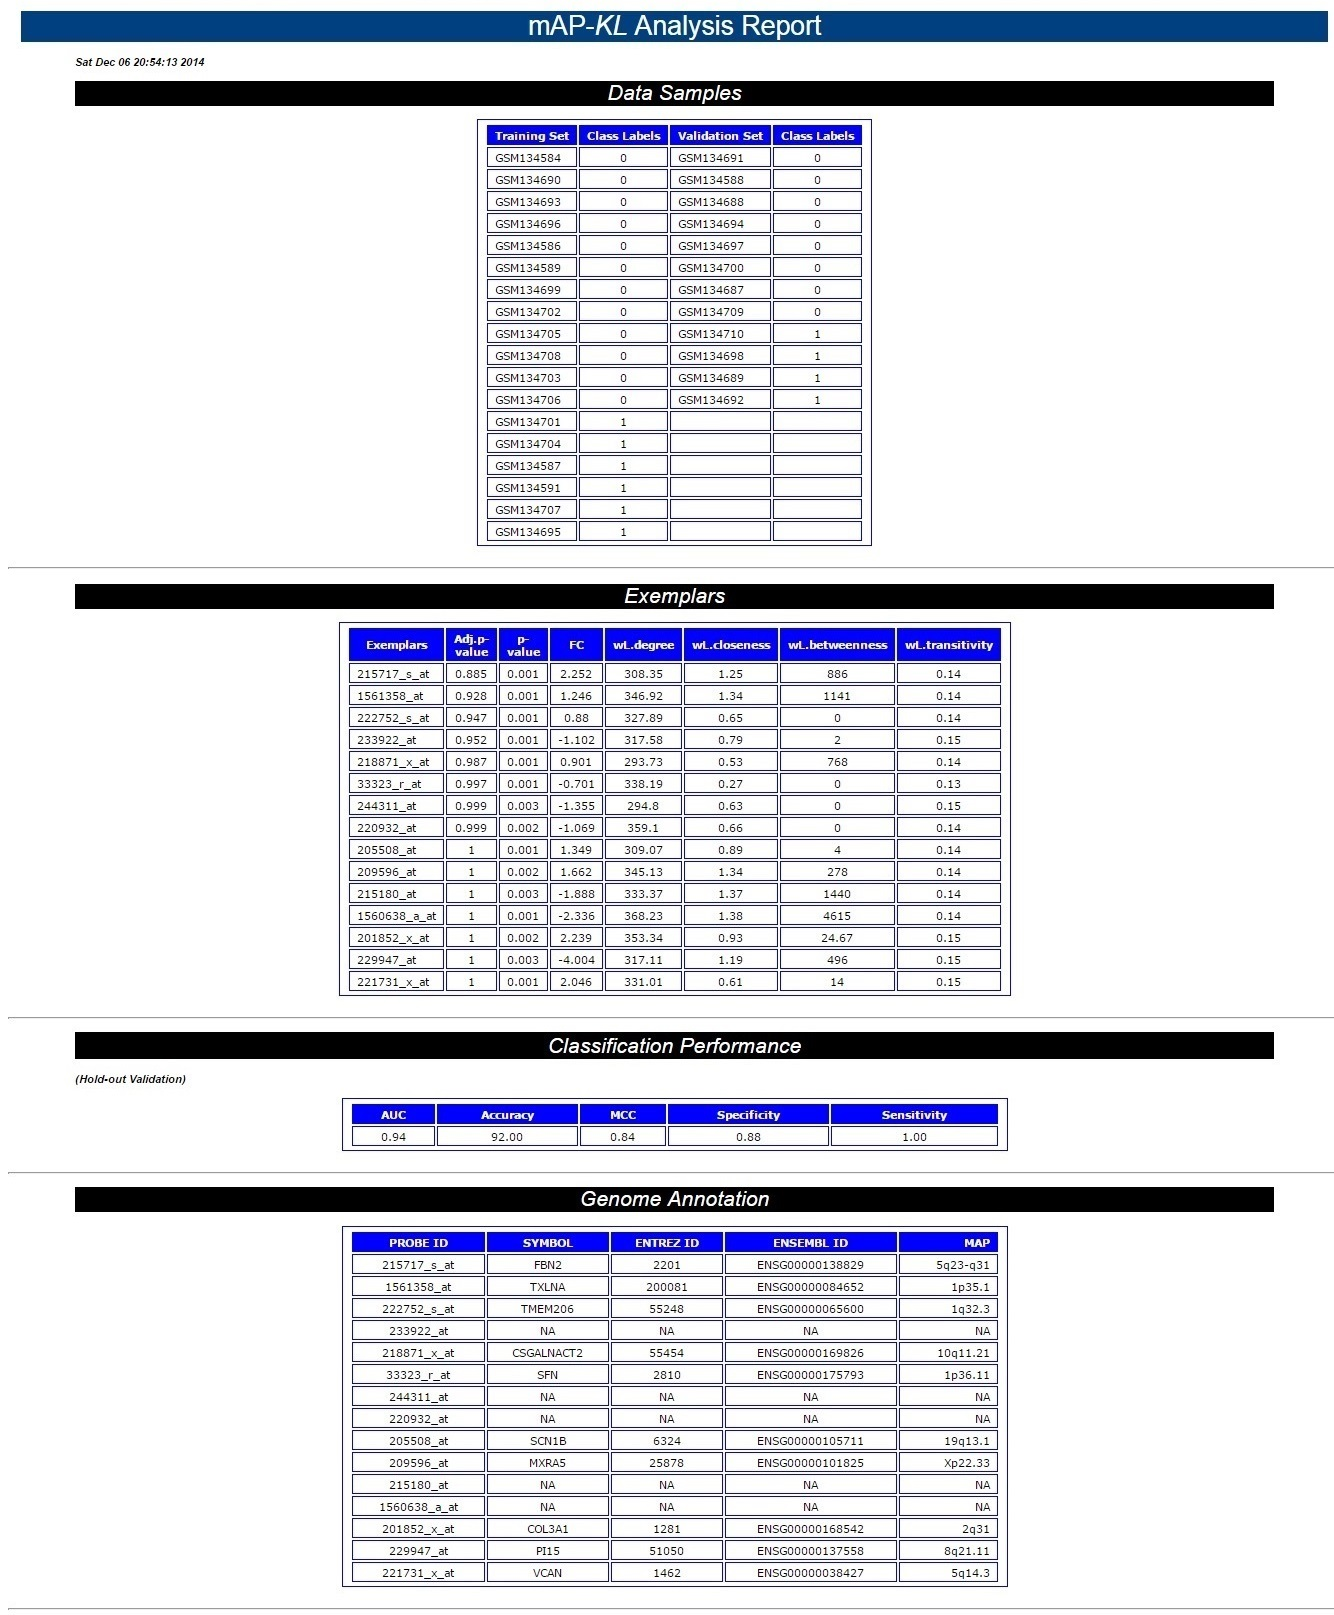
\includegraphics[width=16cm,height=25cm,keepaspectratio]{../man/figures/report}
\caption{mAPKL analysis report}
\end{figure}

\end{document}
